\documentclass[../main/report.tex]{subfiles}
\begin{document}

\chapter{Demolicious}
\label{sec:demolicious}


% Why is the name of our system "Demolicious"?@
% What approach did we take in making a graphics accelerator?@
% What trade-offs did we have to make?@
% What were our concerns?@
% What kind of numbers did we hope to achieve?@

\begin{figure}[htp]
\centering
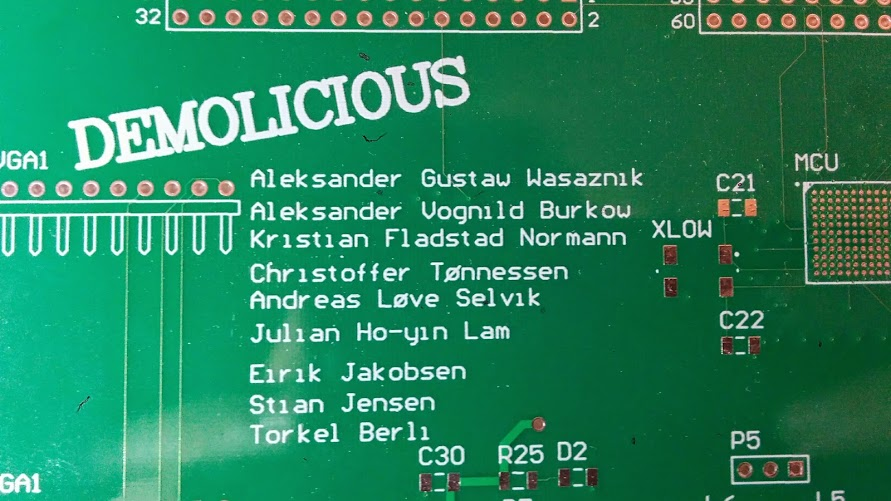
\includegraphics[scale=0.24]{../introduction/assets/PCP_logo.jpg}
\end{figure}

\section{A Graphical Demo Machine}
\label{sec:demolicious-demo-machine}

The system created in this project is named Demolicious.
It is made for running graphical demo's, which is the inspiration for its name.
A graphical demo is a visually pleasing programming feat made to demonstrate the capabilities of the computer as well as the programmer.

Demolicious is inspired by modern PCs' CPU-GPU coordination, both in its programming model and its architectural design.
The CPU will handle programs by default, and offload parallelizable tasks to the GPU.
It will run on a microcontroller.
The GPU will handle parallelizable tasks, like the many graphical operations in a demo, and send graphical data to screen.
Its architecture will be designed and implemented on an FPGA.

Modern GPUs have long development cycles and are very complex.
Demolicious' GPU architecture is necessarily a greatly simplified version.
Because of time constraints, many features that define modern GPUs had to be left out in its design.
The GPU has no branching, and there are no caches.
Modern GPUs have dynamic scheduling to better utilize the resources.
The Demolicious GPU uses barrel processing as a static scheduling scheme, and to hide memory latency.

\section{Demolicious Requirements}

% How did we arrive at our list of requirements?@
For Demolicious to support interesting demos, a set of basic requirements was listed for it.
It certainly needed to display graphics, and a goal was to use HDMI for it.
This decision was partially based on the excitement that it had not been done before in earlier Computer Design Projects, and partially on the fact that it is a modern technology.
Driving video output from the custom GPU was important because a key point of the design was for it to mirror a modern GPU's purpose in a computer system.

Energy efficiency needed to be a primary concern throughout this project.
In an experimental system like Demolicious, that concern will often be sidelined to making anything work in the first place.
Energy efficiency is, after all, an optimization.
Design philosophies like simplicity in GPU architecture and redundancy in PCB options collide somewhat with energy concerns, and both were essential in producing a working system in the short timespan of this project.
One very significant energy optimization for Demolicious made the list of functional goals: setting the CPU to sleep mode when it is idle.

The performance goals were set to be challenging but still reasonable, based on a very rough estimate of potential memory bandwidth and FPGA clock frequency.
Writing interesting demos for the completed machine would be a bonus.
A related bonus would be to write helpful tools to assist in writing the demos.
Table \ref{tab:goals} below lists the initial functional goals, together with priorities, that were decided upon for Demolicious.

\begin{table}[htp]
    \centering
    \begin{tabular}{|p{8cm}|l|}
        \hline
        \textbf{Demolicious Functional Goals}                & \textbf{Priority} \\ \hline
        Demolicious should be general purpose                                   & HIGH    \\ \hline
        Demolicious should display graphics on screen                           & HIGH    \\ \hline
        Demolicious should let its CPU sleep while the GPU executes				& MEDIUM  \\ \hline
        Demolicious should use HDMI for its graphics output	                    & MEDIUM  \\ \hline
        Demolicious should drive video output from its GPU	                    & MEDIUM  \\ \hline
        Demolicious should display a frame of 512 by 256 pixels					& MEDIUM  \\ \hline
        Demolicious should handle an output rate of about 30 frames per second  & MEDIUM  \\ \hline
        Demolicious should have an example application in the form of a visual demo displayed on screen & LOW \\ \hline
        Demolicious should have a toolchain to make life easier for programmers & LOW     \\ \hline
    \end{tabular}
    \caption{Goals set for the Demolicious system}
    \label{tab:goals}
\end{table}

\end{document}
